\section{Overview}
The architecture of uniRDMA is shown in Figure~\ref{fig:framework-overview}. uniRDMA consists of three parts: Verbs libraries in guest, vRNIC (frontend and backend) and management center.

(1) The verbs libraies in guests: They are modified to achive transparency for applications. In specific, we forward the verbs command to uniRDMA frontend. Thus, applications in guest can use verbs libraries same as native RDMA.

(2) vRNIC frontend and backend: Control and data path are separate to achive high-performance. In control path, the vRNIC frontend forwards RDMA verbs to backend in uniRDMA virtual layer, and vRNIC backend execute them; In data path, vRNIC frontend directly use the mapped RDMA resources (e.g. QPs or MRs). The resources are mapped to backend by shared memory.

(3) Management center: To make a centralized management, a management center connect with each host's uniRDMA backend. For example, center configures each vRNIC address, define routing rules and maitain the mapping for vRNIC connections.

\begin{figure}[!ht]
	\centering
	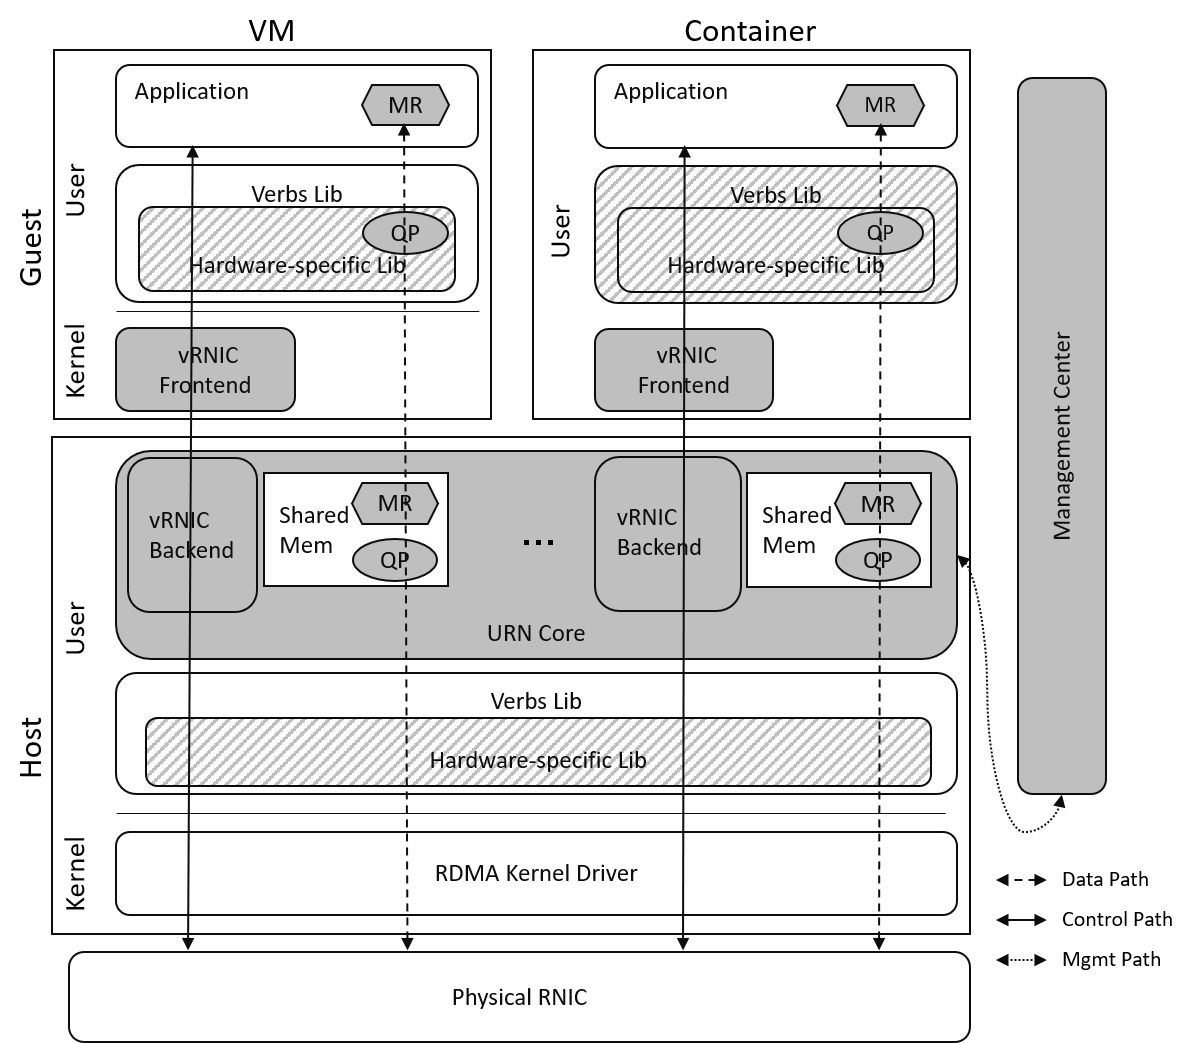
\includegraphics[width=1\linewidth]{images/framework-overview.png}
	\caption{uniRDMA Framework Overview}
	\label{fig:framework-overview}
\end{figure}